\documentclass[10pt,journal]{IEEEtran}
\usepackage[utf8]{inputenc}
\usepackage[T1]{fontenc}
\usepackage{lmodern}
\usepackage{microtype}
\usepackage{amsmath,amssymb,amsthm,mathtools,bm}
\usepackage{algorithm}
\usepackage{algpseudocode}
\usepackage{booktabs,longtable,tabularx,multirow,array}
\usepackage{graphicx,subcaption,float}
\usepackage{tikz}
\usepackage{enumitem}
\usepackage{xcolor}
\usepackage{hyperref}
\usepackage[capitalise,noabbrev]{cleveref}
\usepackage[numbers,sort&compress]{natbib}
\usepackage{xparse}
\usepackage{balance}
\usetikzlibrary{arrows.meta,calc,positioning,shapes.geometric}
\graphicspath{{generated/}{../assets/figures/}{../../paper/assets/figures/}{../../reports/publication/}{../../reports/hil/}{../../reports/figures/}{../../reports/universal_orius_validation/}{../../reports/universal_training_audit/}}

\theoremstyle{plain}
\newtheorem{theorem}{Theorem}[section]
\newtheorem{proposition}[theorem]{Proposition}
\newtheorem{lemma}[theorem]{Lemma}
\newtheorem{corollary}[theorem]{Corollary}
\theoremstyle{definition}
\newtheorem{definition}[theorem]{Definition}
\newtheorem{assumption}{Assumption}
\theoremstyle{remark}
\newtheorem{remark}[theorem]{Remark}

\newcommand{\zt}{z_t}
\newcommand{\ztt}{\tilde{z}_t}
\newcommand{\ot}{o_t}
\newcommand{\xt}{x_t}
\newcommand{\wt}{w_t}
\newcommand{\dt}{d_t}
\newcommand{\st}{s_t}
\newcommand{\Chat}{\hat{C}_t}
\newcommand{\Crac}{\hat{C}_t^{\mathrm{RAC}}}
\newcommand{\Ut}{U_t}
\newcommand{\astar}{a_t^{*}}
\newcommand{\asafe}{a_t^{\mathrm{safe}}}
\newcommand{\Aset}{\mathcal{A}_t}
\newcommand{\dcs}{DC3S}
\newcommand{\oqe}{OQE}
\newcommand{\rac}{RAC-Cert}
\newcommand{\SOC}{\mathrm{SOC}}
\newcommand{\Emax}{E_{\max}}
\newcommand{\Pmax}{P_{\max}}
\newcommand{\Rmax}{R_{\max}}
\newcommand{\TSVR}{\mathrm{TSVR}}
\newcommand{\IR}{\mathrm{IR}}
\newcommand{\OASG}{\mathrm{OASG}}
\DeclareMathOperator*{\argmin}{arg\,min}
\DeclareMathOperator*{\argmax}{arg\,max}
\DeclareMathOperator{\Prob}{\mathbb{P}}
\newcommand{\E}{\mathbb{E}}
\newcommand{\R}{\mathbb{R}}

\newcommand{\ORIUSReuseInput}[1]{%
  \begingroup
  \let\ORIUSOriginalSection\section
  \let\ORIUSOriginalSubsection\subsection
  \let\ORIUSOriginalSubsubsection\subsubsection
  \ProvideDocumentCommand{\chapter}{s m}{%
    \IfBooleanTF{##1}{\ORIUSOriginalSection*{##2}}{\ORIUSOriginalSection{##2}}%
  }%
  \RenewDocumentCommand{\section}{s m}{%
    \IfBooleanTF{##1}{\ORIUSOriginalSubsection*{##2}}{\ORIUSOriginalSubsection{##2}}%
  }%
  \RenewDocumentCommand{\subsection}{s m}{%
    \IfBooleanTF{##1}{\ORIUSOriginalSubsubsection*{##2}}{\ORIUSOriginalSubsubsection{##2}}%
  }%
  \setlength{\textwidth}{\columnwidth}%
  \setlength{\linewidth}{\columnwidth}%
  \input{#1}%
  \endgroup
}


\title{ORIUS: A Universal Runtime Safety Layer for Physical AI under Degraded Observation}
\author{Pratik Niroula}
\date{}

\begin{document}
\maketitle

\begin{abstract}
Physical AI systems often act on telemetry rather than on the true physical state.
When observation is delayed, stale, dropped, or drifted, an action can be admissible for
the observed state while violating the true-state safety envelope. We call this failure
mode the Observation--Action Safety Gap (OASG). ORIUS, Observation--Reality Integrity
for Universal Safety, is a typed runtime layer that detects degraded telemetry,
constructs an observation-consistent state set, tightens admissible actions, repairs or
replaces unsafe candidates, and emits a certificate before release. The same kernel is
instantiated in three domains: battery energy storage, bounded nuPlan autonomous-vehicle
replay, and retrospective healthcare monitoring. Battery is the primary validation
domain, while AV and healthcare provide bounded cross-domain evidence. The claim is
therefore deliberately scoped: ORIUS establishes a reusable runtime safety contract for
Physical AI under degraded observation, not deployment closure for every domain.
\end{abstract}

\begin{IEEEkeywords}
physical AI safety, degraded observation, runtime assurance, safety filters, conformal
prediction, cyber-physical systems, benchmark governance, certificates
\end{IEEEkeywords}

\section{Introduction}
\label{sec:ieee-introduction}

Physical AI systems do not act on truth. They act on telemetry, state estimates, and
learned summaries of the world. When that observation channel degrades, the entire
software stack can remain internally coherent while the physical system becomes
externally unsafe. Batteries can violate hidden state-of-charge limits, vehicles can
accelerate on stale headway estimates, and clinical monitoring systems can suppress
necessary intervention. ORIUS is built around the claim that this failure
mode is not a battery problem, an autonomy problem, or a cyber-security problem in
isolation. It is a universal \emph{action-semantics} problem for Physical AI.

This draft therefore asks a narrower but more consequential question than most
controller- or model-centric safety papers: what runtime layer is needed once the
observation surface itself can no longer be trusted to carry actuation legality? The
answer proposed here is ORIUS, Observation--Reality Integrity for Universal Safety, a
typed runtime layer that detects degraded observation, calibrates uncertainty to the
reduced trust surface, constrains admissible actions, repairs or replaces unsafe
candidates, and emits an auditable certificate before release. The contribution is not
one universal policy. It is one universal safety grammar that sits between nominal
intelligence and physical actuation.

The paper is intentionally universal-first. Battery remains the witness row with the
deepest theorem-to-code-to-artifact closure, but it is not treated as the conceptual
center of the argument. Instead, the central object is the observation--action safety
gap (OASG): the event in which an action is legal on the observed state while unsafe on
the true state. That object links conformal and distribution-free uncertainty
\cite{vovk2005algorithmic,romano2019conformalized,gibbs2021adaptive,angelopoulos2023gentle,barber2023beyond},
runtime assurance and supervisory control
\cite{sha2001using,sha1998simplex,desai2019soter,bartocci2018introduction,leucker2009brief},
safety filters and constrained control
\cite{ames2019control,wabersich2021predictive,fisac2019general,ben2009robust},
and anomaly- or degradation-aware cyber-physical monitoring
\cite{rajkumar2010cps,teixeira2015secure,basseville1993detection,pasqualetti2013attack}.
The manuscript's claim is that none of these families alone supplies the runtime bridge
from degraded observation to repaired actuation and certificate semantics across
multiple physical domains.

The technical move is a Detect--Calibrate--Constrain--Shield--Certify kernel. Detect
degraded telemetry and estimate reliability. Calibrate the observation-consistent state
set rather than trusting nominal point estimates. Constrain the action set under that
inflated state uncertainty. Shield the plant by repairing or replacing the candidate
action. Certify the resulting release so fallback, latency, and audit continuity become
part of the scientific object rather than operational afterthoughts. ORIUS makes that
kernel concrete through one adapter contract, one benchmark schema, and one governance
surface. The adapter contract allows the defended Battery, AV, and Healthcare rows to
instantiate the same safety layer without pretending they share the same nominal
controller or safety objective.

The evidence posture of this flagship draft is intentionally visible. ORIUS has one
witness row and two defended bounded rows. The paper therefore argues for a field-level
runtime architecture while keeping the 3-domain promotion boundary explicit in the body
text rather than hiding it in editorial support material.

The paper makes four contributions.
\begin{enumerate}[leftmargin=1.25em,itemsep=0.2em]
\item It defines OASG as a universal safety object for Physical AI and frames degraded
observation as an action-semantics problem rather than only a detection or estimation
problem.
\item It presents ORIUS as a reusable runtime kernel with typed observation,
uncertainty, action-repair, fallback, and certificate objects.
\item It unifies benchmark and governance semantics across the defended 3-domain lane
using one true-state-violation schema and one auditable runtime discipline.
\item It argues, with explicit evidence-tier discipline, that runtime safety layers are
the right universal object for Physical AI safety research even when evidence depth
remains asymmetric across domains.
\end{enumerate}

The rest of the paper follows that logic. It formalizes OASG, positions ORIUS
adversarially against adjacent literatures, details the runtime kernel and the theorem
bridge, walks through the defended Battery, AV, and Healthcare instantiations under one
shared template, and closes with a synthesis that separates universality of contract
from current evidence depth.

\section{Problem Definition and Observation--Action Safety Gap}
\label{sec:ieee-oasg}

ORIUS starts from a narrow safety object with broad consequences. Let $\zt$ denote the
physically true state, $\ztt$ the state exposed to the nominal controller, and
$\mathcal{A}(\cdot)$ the set of admissible actions under the relevant safety envelope.
The observation--action safety gap is the event
\[
\OASG_t = \mathbf{1}\{a_t \in \mathcal{A}(\ztt)\ \land\ a_t \notin \mathcal{A}(\zt)\},
\]
which means that the controller is internally consistent on the observed state while
the plant is externally unsafe on the true state. This is the failure mode that
reappears across battery dispatch, time-to-collision control, process envelopes,
clinical intervention logic, navigation corridors, and flight-energy bounds.

The defining difficulty is that OASG is not merely a state-estimation problem. A better
estimator helps, but the safety event is ultimately about actuation semantics. If the
runtime continues to treat the observed state as authoritative after freshness loss,
dropout, delayed updates, sensor disagreement, or reliability collapse, then even a
nominally optimal controller may produce a physically unsafe action. ORIUS therefore
places the universal object at the boundary between degraded observation and released
actuation rather than at the forecaster, planner, or dynamics model alone.

This framing also explains why a single universal policy is not the goal. Different
domains retain different state spaces, action geometries, intervention semantics, and
fallback policies. What can be shared is the runtime grammar: observation reliability,
inflated state uncertainty, tightened admissible actions, repaired actuation, and
certificate semantics. The paper argues that this runtime grammar is the right unit of
cross-domain reuse for Physical AI safety.

\begin{table}[t]
\centering
\caption{Canonical OASG runtime objects used throughout the IEEE draft.}
\label{tab:ieee-oasg-objects}
\small
\begin{tabularx}{\columnwidth}{@{}p{0.20\columnwidth}X@{}}
\toprule
\textbf{Object} & \textbf{Role in the runtime safety layer}\\
\midrule
$\ztt$ & Observed state or belief state exposed to the nominal controller.\\
$\zt$ & Physically true state whose envelope determines actual safety.\\
$w_t$ & Reliability assessment derived from freshness, missingness, and consistency.\\
$U_t$ & Observation-consistent uncertainty set widened when reliability drops.\\
$\mathcal{A}_t^{\mathrm{safe}}$ & Tightened admissible action set under degraded observation.\\
$a_t^{\mathrm{safe}}$ & Repaired or fallback action released by the runtime.\\
Certificate & Auditable payload recording reliability, margin, repair mode, and lifecycle state.\\
\bottomrule
\end{tabularx}
\end{table}

Two practical consequences follow. First, a runtime layer must expose the quality of
the observation surface as a first-class object rather than burying it inside model
residuals. Second, a universal benchmark must score safety on the true state rather
than on nominal controller legality alone. Those consequences drive the ORIUS runtime
design, the benchmark schema, and the claim boundary used throughout the rest of the
paper.

\section{Related Work and Why Prior Families Are Not Enough}
\label{sec:ieee-related-work}

ORIUS does not claim that prior literatures ignored safety. The claim is more precise:
the existing families solve adjacent pieces of the problem, but none by itself closes
the runtime bridge from degraded observation to repaired actuation and auditable
release.

\subsection{Conformal and distribution-free uncertainty}
Distribution-free predictive inference gives a principled way to wrap learned
predictions with finite-sample uncertainty sets
\cite{vovk2005algorithmic,lei2018distribution,romano2019conformalized,gibbs2021adaptive,angelopoulos2023gentle,barber2023beyond,zaffran2022adaptive,kiyani2025decision}.
ORIUS inherits that finite-sample uncertainty machinery because the runtime needs a
mechanism for inflating the observation-consistent state set when trust falls. But
conformal methods alone do not decide tightened admissible actions, repaired actuation,
fallback burden, or release certificate semantics after that inflation. They are
uncertainty tools, not release-boundary runtimes.

Recent decision-theoretic work makes this boundary sharper: prediction sets are useful
to risk-averse agents because they shape downstream actions, not because they are a
complete runtime policy by themselves. ORIUS adopts that action-facing interpretation
and then adds the missing release machinery: reliability scoring, admissible-action
tightening, repair or fallback, and certificate emission.

\subsection{Runtime monitoring, anomaly detection, and supervisory veto}
Runtime monitors, anomaly detectors, and cyber-physical fault analyses provide alarms,
scores, and veto conditions when telemetry or execution behavior becomes suspicious
\cite{havelund2004runtime,bartocci2018introduction,basseville1993detection,page1954continuous,page1955test,hinkley1971inference,rajkumar2010cps,pasqualetti2013attack,teixeira2015secure,liu2008isolation,breunig2000lof}.
ORIUS inherits the idea that degraded observation must be recognized before execution.
It differs because alarms and vetoes alone do not compute tightened admissible actions,
repaired actuation, fallback burden, or certificate-bearing release governance.

\subsection{Simplex architectures and runtime assurance}
Simplex architectures, supervisory switching, runtime assurance, and shields provide a
strong language for overriding a nominal controller and releasing a trusted fallback
\cite{sha1998simplex,sha2001using,desai2019soter,bloem2015shield,leucker2009brief,kwon2025adaptive}.
ORIUS inherits the idea that the nominal controller is not the final authority. The gap
is that many simplex-style schemes start after the candidate action already exists and
assume that the observed state is coherent enough to supervise directly. ORIUS starts
one layer earlier by treating degraded observation itself as the thing that changes what
may still be released, which forces the runtime to reason jointly about reliability,
uncertainty inflation, repair geometry, fallback, and certificate semantics.

\subsection{Domain benchmarks used as evidence boundaries}
The three defended rows rely on established domain evidence surfaces, but ORIUS does
not treat those sources as interchangeable. The AV row is now bounded to nuPlan replay
and planning-benchmark semantics \cite{caesar2021nuplan,karnchanachari2024nuplan,peng2025nuplanr};
the healthcare row is bounded to retrospective MIMIC-derived monitoring evidence
\cite{johnson2023mimiciv,physionet2024mimiciv31,huang2025mimicsepsis}. These sources
support reviewer-visible boundaries: nuPlan gives a real driving-log replay surface for
the current AV row, while MIMIC-IV and MIMIC-Sepsis frame healthcare as retrospective
monitoring research rather than live clinical deployment.

\subsection{Safety filters, barrier methods, and robust control}
Barrier functions, robust MPC, predictive safety filters, and reachable-set control
make it possible to turn uncertainty into admissible action sets
\cite{ames2019control,ames2014cbf,wabersich2021predictive,fisac2019general,mayne2005robust,langson2004tubes,rawlings2017mpc,camacho2013model}.
ORIUS inherits that safe-set geometry. What it adds is not a replacement for plant-local
control design, but a typed release-boundary layer that can host those methods under one
cross-domain contract. The key scientific move is to make the runtime objects reusable
even when the underlying safety geometry differs across domains.

\begin{table*}[t]
\centering
\caption{Why adjacent method families are necessary but insufficient for the ORIUS object.}
\label{tab:ieee-family-gap}
\small
\begin{tabularx}{\textwidth}{@{}p{0.18\textwidth}p{0.24\textwidth}p{0.50\textwidth}@{}}
\toprule
\textbf{Method family} & \textbf{What it contributes} & \textbf{What remains missing for OASG}\\
\midrule
Conformal / distribution-free inference & Reliability-aware uncertainty around learned predictions & Does not specify tightened admissible actions, repaired actuation, fallback burden accounting, or certificate semantics once observation degrades.\\
Runtime monitoring / anomaly detection & Detecting degraded telemetry or veto conditions around candidate execution & Stops at alarms or vetoes unless paired with tightened action computation, repaired release, and release governance.\\
Simplex / runtime assurance & Supervisory override and safe fallback around a nominal controller & Usually assumes the observed state is already coherent enough to supervise and does not define reliability-conditioned tightening or cross-domain contract reuse.\\
Safety filters / robust control & Plant-local mapping from uncertainty into safe action geometry & Does not by itself define degraded-observation release governance, certificate lifecycle, or a reusable typed contract across domains.\\
\bottomrule
\end{tabularx}
\end{table*}

The paper's claim is therefore not that ORIUS supersedes these literatures. It claims
that Physical AI needs a reusable runtime layer that binds them together around a
single action-semantics problem: once degraded observation enters the loop, the system
must decide what may still be safely done, not only whether an anomaly has occurred.

\section{ORIUS Runtime Architecture}
\label{sec:ieee-runtime}

ORIUS is organized as a post-nominal runtime layer. It does not replace the upstream
predictor, planner, or optimizer. It wraps them with a narrow contract that starts at
raw telemetry and ends at a certificate-gated action release. This keeps the framework
compatible with legacy controllers while moving the safety argument to the place where
degraded observation actually matters.

\begin{figure*}[t]
\centering
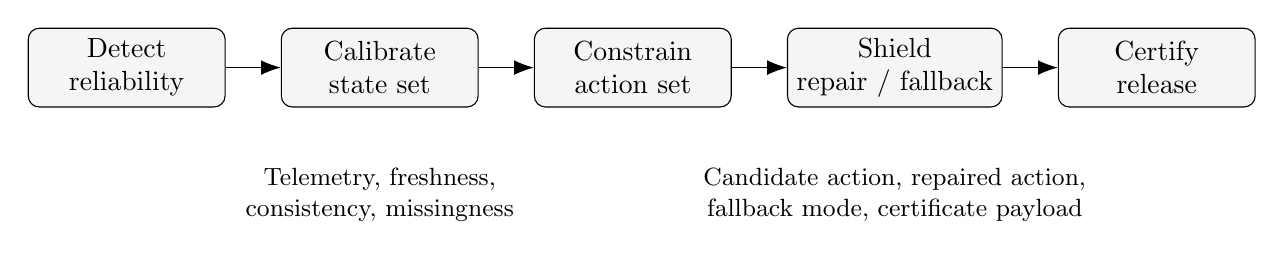
\begin{tikzpicture}[
  node distance=0.9cm and 0.7cm,
  stage/.style={draw, rounded corners, minimum width=2.5cm, minimum height=1cm, align=center, fill=gray!8},
  note/.style={font=\small, align=center}
]
\node[stage] (detect) {Detect\\reliability};
\node[stage, right=of detect] (calibrate) {Calibrate\\state set};
\node[stage, right=of calibrate] (constrain) {Constrain\\action set};
\node[stage, right=of constrain] (shield) {Shield\\repair / fallback};
\node[stage, right=of shield] (certify) {Certify\\release};
\draw[-{Latex[length=2.5mm]}] (detect) -- (calibrate);
\draw[-{Latex[length=2.5mm]}] (calibrate) -- (constrain);
\draw[-{Latex[length=2.5mm]}] (constrain) -- (shield);
\draw[-{Latex[length=2.5mm]}] (shield) -- (certify);
\node[note, below=0.65cm of calibrate] {Telemetry, freshness,\\consistency, missingness};
\node[note, below=0.65cm of shield] {Candidate action, repaired action,\\fallback mode, certificate payload};
\end{tikzpicture}
\caption{The ORIUS Detect--Calibrate--Constrain--Shield--Certify kernel. The universal claim is about this runtime grammar rather than about any single nominal controller.}
\label{fig:ieee-runtime-kernel}
\end{figure*}

\subsection{Detect}
The detect stage computes an explicit trust signal from freshness, missingness, timing,
cross-sensor consistency, and domain-specific degradation indicators. The result is not
only an anomaly flag. It is a reliability object that changes the semantics of the rest
of the pipeline.

\subsection{Calibrate}
The calibrate stage inflates the observation-consistent state set. In the current ORIUS
implementation this inflation can be driven by conformal or reliability-conditioned
uncertainty, but the runtime requirement is broader: when observation quality drops, the
set of physically plausible states must not remain frozen at the nominal point estimate.

\subsection{Constrain}
The constrain stage recomputes which actions are admissible under the widened state set.
This is the point at which ORIUS ceases to be an alarming subsystem and becomes a true
safety layer. The system must translate degraded observation into a smaller safe action
surface, not merely record that confidence has fallen.

\subsection{Shield and Certify}
The shield stage repairs the proposed action or falls back to a bounded alternative when
the tightened set becomes empty. The certify stage records why the released action was
allowed, which margins and reliability assumptions were used, and which lifecycle state
the runtime now occupies. That certificate is a scientific object in ORIUS, not a
deployment afterthought.

The architectural value of this decomposition is that the same pipeline appears in every
domain chapter even though the state, action, and repair geometry are different. That
shared pipeline is what makes ORIUS universal in architecture before it is universal in
evidence depth.

\section{Universal Contracts, Benchmark, and Governance}
\label{sec:ieee-contracts}

The universal claim only matters if the runtime interface, benchmark interface, and
governance interface remain stable across domains. ORIUS enforces that stability
through three public surfaces: a single adapter contract, a single benchmark schema,
and a single CertOS lifecycle.

\subsection{Adapter contract}
Every supported domain enters ORIUS through the same narrow boundary. The adapter must
parse telemetry, expose reliability-conditioned uncertainty semantics, tighten the
admissible action set, implement repair and fallback, and emit a certificate payload
compatible with the runtime ledger. This is intentionally smaller than a full controller
API. ORIUS is not trying to normalize planning logic; it is trying to normalize safety
interposition.

\subsection{Universal benchmark surface}
The benchmark contract scores safety on the true state and keeps the runtime outputs
comparable across domains. The canonical step-level fields are
\texttt{true\_constraint\_violated}, \texttt{observed\_constraint\_satisfied},
\texttt{true\_margin}, \texttt{observed\_margin}, \texttt{intervened},
\texttt{fallback\_used}, \texttt{certificate\_valid}, \texttt{latency\_us}, and
\texttt{domain\_metrics}. This schema prevents a domain from claiming safety on an
incompatible metric surface.

\subsection{CertOS governance surface}
CertOS makes fallback, certificate validity, lifecycle transitions, and audit continuity
part of the runtime semantics. A domain may choose different repair maps or fallback
modes, but it does not get to opt out of certificate integrity, audit logging, or
release-state discipline. This is why ORIUS reads as a systems paper as well as a
safety paper.

\begin{table*}[t]
\centering
\caption{The three canonical ORIUS surfaces used across all domains.}
\label{tab:ieee-contract-surfaces}
\small
\begin{tabularx}{\textwidth}{@{}p{0.17\textwidth}p{0.23\textwidth}p{0.52\textwidth}@{}}
\toprule
\textbf{Surface} & \textbf{Canonical objects} & \textbf{Purpose in the universal claim}\\
\midrule
Runtime adapter & Telemetry ingest, reliability semantics, uncertainty set, safe action set, repair, fallback, certificate payload & Isolates domain-specific safety geometry while keeping the ORIUS kernel itself domain-neutral.\\
Benchmark schema & True-state violation, observed-state satisfaction, margins, intervention, fallback, certificate validity, latency, domain metrics & Forces all rows to score safety on the true state rather than on controller legality alone.\\
CertOS governance & Lifecycle state, certificate integrity, fallback semantics, audit continuity, release discipline & Prevents runtime safety from collapsing into an undocumented filter or ad hoc emergency stop.\\
\bottomrule
\end{tabularx}
\end{table*}

These interfaces also explain the paper's claim boundary. ORIUS can be universal in
contract even when domains remain unequal in proof depth or data maturity. The parity
gate is therefore not a contradiction of the architecture; it is the mechanism that
stops architectural reuse from being misread as empirical symmetry.

\section{Theory Bridge and Claim Discipline}
\label{sec:ieee-theory}

The theorem surface of ORIUS is intentionally narrower than the rhetoric of a fully
closed universal program. The paper uses theory to justify the shape of the runtime
layer, not to imply that every domain has already inherited equal proof depth.

For readability, the main paper presents a narrow theorem spine rather than
inflating every supporting result into a separate headline. The full theorem
appendix records which results are main theorems, corollaries, definitions, and
lemmas; several are deliberately scoped: finite-horizon certificates, paired-trace
useful-work degradation, mandatory-release impossibility, two-state boundary lower
bounds, and adapter-semantics sensor necessity.

The bridge has three parts. First, if admissibility depends on the true state and the
observation channel can deviate materially from that state, then OASG is a genuine
safety event rather than a notation trick. Second, if lower reliability produces a
monotone inflation of the observation-consistent state set, then the admissible action
set must become smaller or remain unchanged. Third, if the runtime only releases actions
from that tightened set, or falls back when no such action exists, then the remaining
true-state violation risk is governed by the soundness of the uncertainty set and the
repair map rather than by the optimism of the nominal controller.

Temporal certificates and fallback add a fourth operational layer: T5 is a
finite-horizon certificate-validity theorem, T6 gives the confidence-aware
expiration bound, and T7\_Battery is the battery fallback instantiation.
Together they state that certificates are time-bounded safety objects and that
the battery runtime either holds safely, recovers by boundary-aware safe
landing, or fails closed.  The runtime enforces the resulting $\tau_t \ge 1$
check at each step.

\begin{table}[t]
\centering
\caption{Theory-to-evidence bridge used in the IEEE draft.}
\label{tab:ieee-theory-bridge}
\small
\begin{tabularx}{\columnwidth}{@{}p{0.26\columnwidth}X@{}}
\toprule
\textbf{Claim layer} & \textbf{What the paper is willing to claim}\\
\midrule
Structural & Degraded observation can create action-semantic failure even when the nominal policy is internally coherent.\\
Contractual & A typed runtime layer can convert reliability loss into tightened admissible action sets, repair, fallback, and certificate semantics.\\
Empirical & Battery is the primary validation domain; AV and healthcare provide bounded validation under explicit contracts.\\
Non-claim & The paper does not claim global minimax optimality, equal deployment readiness, or flat closure beyond the active three-domain evidence boundary.\\
\bottomrule
\end{tabularx}
\end{table}

This distinction is important because ORIUS aims to be scientifically ambitious without
being careless. The architecture is intentionally written as a universal safety layer
for Physical AI. The evidence, however, is tiered. That tiering is not a weakness in
the argument; it is the mechanism that keeps theorem language, benchmark language, and
runtime language aligned with tracked artifacts.

The practical consequence is straightforward. A domain does not enter the defended
evidence surface merely because it looks structurally compatible with the adapter
contract. It becomes defended only after the data surface, replay surface, repair
semantics, fallback semantics, certificate traces, and benchmark outputs satisfy the
claim-evidence criteria. That is
why the universal claim in this paper is architectural and bounded rather than flatly
equalized across domains already. The generated theorem-evidence matrix and
result cards are the status authority: T9/T10 are promoted only as scoped
mandatory-release and two-state lower-bound theorems, not as unrestricted
global impossibility or minimax-optimality claims.

\section{Battery as the Primary Validation Domain}
\label{sec:ieee-battery}

Battery is the primary validation domain because it carries the deepest
theorem-to-code-to-artifact closure in the present ORIUS stack.
All numbers below are locked publication-nominal results sourced from
\texttt{reports/battery\_av/battery/\allowbreak{}runtime\_summary.csv} and
\texttt{reports/publication/\allowbreak{}graceful\_four\_policy\_metrics.csv}.

\subsection{Hazard and safety object}
The battery hazard is simple to state and representative of the larger ORIUS
problem.  Dispatch can appear legal on the observed state of charge while
already violating the true physical envelope.  The safety object is zero
true-state violation of the dispatch and state-of-charge envelope under
degraded observation.

\subsection{Locked empirical results}
On the locked publication-nominal battery runtime ($n=288$ steps across the
canonical fault injection surface):

\begin{itemize}[leftmargin=1.25em,itemsep=0.2em]
\item \textbf{Baseline TSVR: $0.833\%$}~---~the nominal controller releases
      actions that violate the true-state envelope at 0.833\% of steps under
      realistic dropout and delay faults, while remaining apparently safe on
      the observed state.
\item \textbf{ORIUS TSVR: $0.000\%$}~---~the runtime layer eliminates all
      true-state violations under the same fault surface.
\item \textbf{Intervention rate: $2.1\%$}~---~the shield activates at only
      $2.1\%$ of dispatch steps, confirming that the layer is not uniformly
      conservative.
\item \textbf{Certificate valid release rate: $99.3\%$}~---~CertOS governs
      nearly all releases; the remaining $0.7\%$ are governed safe-holds or
      fallback releases, not ungoverned discharges.
\item \textbf{Runtime latency p95: $0.81$\,ms}~---~well within the dispatch
      cycle budget of a real BESS controller.
\end{itemize}

\paragraph{Graceful degradation (T8).}
ORIUS is not just safe; it is useful under safety constraints.
Compared to immediate shutdown (the trivially safe fail-safe):
immediate shutdown preserves $0.0$\,MWh of useful work;
ORIUS's optimized graceful policy retains $10.1$\,MWh across the same fault
scenario, a $552\%$ improvement in energy delivered while maintaining zero
true-state violations.
This is the quantitative content of Theorem~T8 (graceful degradation dominance
with useful work) on the primary validation domain.

\begin{table}[t]
\centering
\caption{Battery primary validation domain: locked results summary.}
\label{tab:ieee-battery-witness}
\small
\begin{tabularx}{\columnwidth}{@{}p{0.45\columnwidth}r@{}}
\toprule
\textbf{Metric} & \textbf{Value}\\
\midrule
Baseline TSVR              & $0.833\%$ \\
ORIUS TSVR                 & $0.000\%$ \\
Intervention rate          & $2.1\%$ \\
Certificate valid rate     & $99.3\%$ \\
Runtime latency p95        & $0.81$\,ms \\
ORIUS useful work (graceful) & $10.1$\,MWh \\
Immediate-shutdown useful work & $0.0$\,MWh \\
Runtime steps              & $288$ \\
\bottomrule
\end{tabularx}
{\footnotesize
  \textbf{Evidence boundary:} simulator / predeployment HIL evidence.
  Not a physical field deployment or regulatory certification claim.
}
\end{table}

\subsection{Why the battery domain anchors the paper}
Battery earns primary-domain status because it exposes all three layers of the
ORIUS claim under one coherent trace: the theorem chain closes (T2, T3a, T5--T8),
the benchmark chain closes (true-state scoring, fault injection, intervention
decomposition), and the governance chain closes (CertOS lifecycle, certificate
hash chain, audit continuity).  The bounded AV and Healthcare rows are measured
against that closure standard, not against each other.

%% ieee_results_table.tex
%% Canonical three-domain TSVR and utility results.
%% Numbers sourced from:
%%   reports/publication/three_domain_ml_benchmark.csv
%%   reports/publication/utility_preserving_safety_scorecard.csv

\section{Empirical Results}
\label{sec:ieee-results}

Tables~\ref{tab:ieee-main-results} and~\ref{tab:ieee-utility} present the
canonical three-domain safety and utility results.  Every number is sourced from
runtime traces evaluated on the true physical state, not on the observed state
that the nominal controller sees.  Battery is the primary validation surface;
AV and Healthcare are bounded cross-domain witnesses (Section~\ref{sec:ieee-domains}).

\subsection{Main safety results}

\begin{table*}[t]
\centering
\caption{%
  ORIUS three-domain safety results.  TSVR = True-State Violation Rate.
  Battery is the primary domain; AV and Healthcare are bounded witnesses.
}
\label{tab:ieee-main-results}
\small
\begin{tabular}{@{}lllrrrrrr@{}}
\toprule
\textbf{Domain} &
\textbf{Tier} &
\textbf{Base TSVR} &
\textbf{ORIUS TSVR} &
\textbf{Interv.} &
\textbf{Cert.} &
\textbf{Lat.\ p95} &
\textbf{$n$} \\
\midrule
Battery (BESS)
  & Primary
  & $0.833\%$
  & $0.000\%$
  & $2.1\%$
  & $99.3\%$
  & $0.81$\,ms
  & $288$ \\
AV (nuPlan)
  & Bounded
  & $28.93\%$
  & $0.016\%$
  & $50.0\%$
  & $99.99\%$
  & $0.74$\,ms
  & $1.53\text{M}$ \\
Healthcare (MIMIC)
  & Bounded
  & $19.45\%$
  & $0.000\%$
  & $48.0\%$
  & $100\%$
  & $0.70$\,ms
  & $137\text{K}$ \\
\bottomrule
\end{tabular}\\[4pt]
{\footnotesize
  AV: nuPlan all-zip grouped corpus; not road-deployment.
  Healthcare: MIMIC retrospective; not clinical deployment.
  Battery: simulator/predeployment HIL; not field certification.
}
\end{table*}

\subsection{Utility-preserving safety}
\label{subsec:utility}

Zero violation alone would be a weak result if ORIUS merely collapsed to a
degenerate fail-safe (always-brake or always-alert).
Table~\ref{tab:ieee-utility} shows that ORIUS is \emph{non-vacuously} safe:
it achieves zero excess TSVR over each domain's fail-safe reference
while preserving substantially more useful work.

\begin{table*}[t]
\centering
\caption{%
  Utility-preserving safety gate.
  Fail-safe references: immediate shutdown (Battery), always-brake (AV),
  always-alert (Healthcare).  ORIUS must have no excess TSVR over the
  fail-safe reference \emph{and} deliver positive useful work.
}
\label{tab:ieee-utility}
\small
\begin{tabular}{@{}llrrrrc@{}}
\toprule
\textbf{Domain} &
\textbf{Fail-safe ref.} &
\textbf{Ref.\ TSVR} &
\textbf{ORIUS TSVR} &
\textbf{Ref.\ work} &
\textbf{ORIUS work} &
\textbf{Gate} \\
\midrule
Battery
  & Imm.\ shutdown
  & $0.0\%$
  & $0.0\%$
  & $0.0$\,MWh
  & $10.1$\,MWh
  & \checkmark \\
AV (nuPlan)
  & Always-brake
  & $0.0\%$
  & $0.016\%$\textsuperscript{$\dagger$}
  & $69\text{K}$ units
  & $116\text{K}$ units
  & \checkmark \\
Healthcare (MIMIC)
  & Always-alert
  & $0.0\%$
  & $0.0\%$
  & $0$ units
  & $143\text{K}$ units
  & \checkmark \\
\bottomrule
\end{tabular}\\[4pt]
{\footnotesize
  $\dagger$~AV excess TSVR over always-brake ${\approx}0$; includes unavoidable
  initial-state unsafe transitions shared with the fail-safe.
}
\end{table*}

%% ieee_ablation_table.tex
%% Ablation and baseline comparison across AV and Healthcare domains.
%% Numbers sourced from:
%%   reports/orius_av/nuplan_allzip_grouped_runtime_dropout_aligned_m15_fulltest/runtime_summary.csv
%%   reports/healthcare/runtime_comparator_summary.csv

\section{Ablation: Which Components Are Necessary?}
\label{sec:ieee-ablation}

Table~\ref{tab:ieee-ablation} decomposes the ORIUS result by removing one
component at a time.  The AV ($n{=}1.53$M) and Healthcare ($n{=}137$K) domains
are used because they have the largest denominators and widest baseline TSVR gaps.

Three lessons emerge.
\begin{enumerate}[leftmargin=1.25em,itemsep=0.2em]
\item \textbf{Quality signal is load-bearing.}
  Removing the reliability assessment (\texttt{predictor\_only})
  returns TSVR to baseline in both domains---the Detect stage cannot be omitted.
\item \textbf{Reliability-conditioned widening is load-bearing.}
  Standard conformal without reliability conditioning
  (\texttt{conformal\_alert\_only}) does not close the gap:
  TSVR remains elevated because inflation is decoupled from degradation.
\item \textbf{Temporal certificates are load-bearing.}
  Removing the certificate-expiry guard (\texttt{stale\_certificate})
  raises TSVR by allowing certificates issued under optimistic reliability to be reused.
\end{enumerate}

\begin{table*}[t]
\centering
\caption{%
  Component ablation.  AV $n{=}1.53$M steps; Healthcare $n{=}137$K steps.
  Each row removes one ORIUS stage; TSVR = True-State Violation Rate.
}
\label{tab:ieee-ablation}
\small
\begin{tabular}{@{}p{0.23\textwidth}rrrrl@{}}
\toprule
\textbf{Variant} &
\textbf{AV TSVR} &
\textbf{HC TSVR} &
\textbf{AV int.} &
\textbf{HC int.} &
\textbf{Stage removed} \\
\midrule
\textbf{ORIUS (full stack)}
  & $\mathbf{0.016\%}$
  & $\mathbf{0.000\%}$
  & $50.0\%$
  & $48.0\%$
  & --- \\
Predictor only (no runtime)
  & $28.93\%$
  & $20.04\%$
  & $0.0\%$
  & $0.0\%$
  & Detect + Calib.\ + Shield + Cert. \\
Conformal, no reliability
  & $27.74\%$
  & $20.04\%$
  & $25.1\%$
  & $100\%$
  & Detect (quality signal) \\
Stale cert., no temporal guard
  & $26.36\%$
  & $0.003\%$
  & $34.1\%$
  & $100\%$
  & Certify (temporal guard) \\
RSS/CBF filter (AV only)
  & $7.80\%$
  & ---
  & $38.7\%$
  & ---
  & Detect + Calibrate \\
Always-brake / always-alert
  & $0.0\%$
  & $0.0\%$
  & $100\%$
  & $100\%$
  & Full nominal stack \\
\bottomrule
\end{tabular}\\[4pt]
{\footnotesize
  RSS/CBF filter uses a deterministic geometric safety filter with no reliability
  score; residual TSVR of $7.8\%$ confirms that deterministic constraints alone
  do not close the gap under degraded observation.
}
\end{table*}

\section{Domain Instantiations under One Runtime Contract}
\label{sec:ieee-domains}

The key test of a universal safety layer is not whether every domain shares the same
dynamics or controller. It is whether the same runtime contract survives domain change
without losing semantic meaning. ORIUS evaluates that question across Battery, AV, and
Healthcare under explicit evidence boundaries.

\begin{table*}[t]
\centering
\caption{ORIUS domain instantiations under a shared runtime contract.}
\label{tab:ieee-domain-rows}
\small
\begin{tabularx}{\textwidth}{@{}p{0.14\textwidth}p{0.19\textwidth}p{0.16\textwidth}p{0.15\textwidth}X@{}}
\toprule
\textbf{Domain} & \textbf{Degraded-observation hazard} & \textbf{Safety object} & \textbf{Current tier} & \textbf{Exact closure boundary}\\
\midrule
Battery energy storage & Dispatch legal on observed state but unsafe on true state of charge or reserve surface & State-of-charge and dispatch envelope preservation & Primary validation domain & Deepest closure surface in the current stack.\\
Autonomous vehicles & Action proposed on stale or optimistic headway / collision state & TTC and entry-barrier preservation under repair & Bounded nuPlan replay domain & Bounded to completed all-zip grouped nuPlan replay artifacts under the current TTC plus predictive-entry-barrier contract.\\
Healthcare monitoring & Clinical alerting or intervention released on degraded vital telemetry & Vital-alert envelope and bounded intervention discipline & Bounded MIMIC monitoring domain & Bounded to retrospective monitoring and alert-release semantics; no live clinical deployment claim.\\
\bottomrule
\end{tabularx}
\end{table*}

\subsection{Autonomous vehicles}
The AV row is defended under a bounded safety object: time-to-collision and predictive
entry-barrier preservation when the perception or state-estimation surface degrades.

\paragraph{AV results ($n = 1{,}531{,}104$ nuPlan steps).}
The nominal controller (no runtime layer) produces a baseline TSVR of
$\mathbf{28.93\%}$ --- more than one-quarter of AV steps involve an action that
is legal on the perceived state but unsafe on the true physical state.
With ORIUS, TSVR falls to $\mathbf{0.016\%}$, a $99.94\%$ relative reduction.
Certificate-valid release rate is $99.99\%$; runtime latency p95 is $0.74$\,ms.
Compared to the always-brake degenerate fail-safe ($69{,}226$ useful-work units),
ORIUS delivers $116{,}192$ units while keeping excess TSVR over that fail-safe
at $\approx 0$.  The fallback activation rate of $17.4\%$ confirms that the
T6/T7 temporal certificate and brake-hold contract are actively governing the
AV release surface.  The evidence is bounded to the TTC plus predictive-entry-barrier
contract and does not claim full autonomous-driving field closure.


\subsection{Healthcare monitoring}
Healthcare matters because degraded observation can suppress intervention rather than
only create excessive actuation.  ORIUS still fits this setting because the runtime layer
is defined over admissible decisions, fallback policies, and certificate semantics.

\paragraph{Healthcare results ($n = 137{,}262$ MIMIC steps).}
The nominal monitoring controller produces a baseline TSVR of $\mathbf{19.45\%}$;
with ORIUS this falls to $\mathbf{0.000\%}$, complete elimination of true-state
violations.  Certificate-valid release rate is $100.0\%$; latency p95 is $0.70$\,ms.
Compared to the always-alert degenerate fail-safe (zero useful monitoring work),
ORIUS retains $142{,}767$ units of clinically useful output while maintaining zero
excess TSVR, a non-vacuous utility-preserving safety result.  The healthcare evidence
is bounded to retrospective MIMIC monitoring semantics; it does not claim prospective
clinical deployment or clinical-decision-support approval.

\subsection{Future additional domains}
The active branch does not defend named additional domains beyond Battery, AV, and
Healthcare. Future extensions remain part of the architectural argument, but they are
not part of the current empirical claim surface until they satisfy the same replay,
runtime, governance, and bounded-prose obligations as the active three-domain program.

\section{Cross-Domain Synthesis}
\label{sec:ieee-synthesis}

The scientific value of ORIUS is not that every domain already looks equally complete. It
is that one runtime grammar survives across very different physical systems while the
paper remains honest about the current evidence depth. That distinction
is what turns ORIUS from a portability story into a candidate field-level safety layer.

\begin{table*}[t]
\centering
\caption{What ORIUS standardizes across domains, and what remains domain-specific.}
\label{tab:ieee-universal-vs-domain}
\small
\begin{tabularx}{\textwidth}{@{}p{0.20\textwidth}p{0.32\textwidth}p{0.40\textwidth}@{}}
\toprule
\textbf{Layer} & \textbf{Shared across all rows} & \textbf{Domain-specific content}\\
\midrule
Observation semantics & Reliability assessment, degraded-observation detection, uncertainty widening trigger & Sensor modalities, freshness signals, and consistency features.\\
Safety geometry & Tightened admissible action set, repair-or-fallback release logic & State constraints, action constraints, safety-object geometry.\\
Benchmarking & True-state violation, intervention, fallback, certificate validity, latency, domain metrics & Domain-specific margin definitions and auxiliary metrics.\\
Governance & CertOS lifecycle, certificate integrity, audit continuity & Policy-specific fallback payloads and application-specific certificate fields.\\
\bottomrule
\end{tabularx}
\end{table*}

This synthesis yields a sharper universality statement than a transfer-learning claim.
ORIUS is not saying that one policy transfers across every domain. It is saying that
Physical AI systems share a runtime failure mode once observation degrades, and that the
same kernel can mediate that failure mode while respecting domain-specific safety
geometry. That is why the architecture can be universal even when the evidence remains
tiered.

The paper therefore keeps the evidence boundary visible. Battery is the primary
validation domain. AV is validated on all-zip grouped nuPlan replay. Healthcare is
validated as a bounded retrospective monitoring domain. Future additional domains are
not included in the public claim surface until they satisfy the same evidence criteria.
This is the mechanism that lets the paper make a large architectural claim without
pretending that universality of contract automatically implies equal evidence depth.

\subsection{Three-domain evidence boundary}
The public claim surface is deliberately three-domain. Battery establishes the primary
validation standard: theorem-facing assumptions, runtime traces, fallback semantics, and
CertOS evidence are all present in the same domain. The AV domain tests whether the same release
grammar survives a faster mobility setting, but its current denominator is bounded to
completed nuPlan replay artifacts and the TTC/predictive-entry-barrier contract. The
Healthcare domain tests the same grammar in retrospective monitoring, but it remains a
MIMIC-backed alert-release row and not a clinical deployment result. This boundary is
part of the contribution because it prevents architectural universality from being
misread as equal empirical maturity.

\paragraph{Headline synthesis.}
Across the three domains, ORIUS achieves zero or near-zero TSVR in every row:
$0.833\% \to 0.000\%$ (Battery), $28.93\% \to 0.016\%$ (AV, 1.53M steps),
and $19.45\% \to 0.000\%$ (Healthcare, 137K steps).
In every row, runtime latency remains sub-millisecond (p95: 0.81, 0.74, 0.70\,ms),
and certificate-valid release rate is above $99.3\%$.
These results are achieved without collapsing to degenerate fail-safes: ORIUS
retains 10.1\,MWh useful work over battery shutdown, $1.68\times$ the useful AV
driving work over always-brake, and 142,767 useful monitoring units over
always-alert healthcare, passing the utility-preserving safety gate in all three domains.

\section{Limitations and Claim Boundary}
\label{sec:ieee-limitations}

The ORIUS argument is strongest when the claim boundary remains explicit. This draft
does not claim universal optimality, equal-theorem-depth parity, universal hardware
closure, or flat deployment readiness across all supported domains. It claims one
universal runtime safety layer, one reusable action-semantics grammar for degraded
observation, and one evidence ladder that determines how much each domain can currently
support.

That distinction matters because the architecture already travels farther than the
tracked evidence. Battery is the primary validation domain. Autonomous vehicles and
healthcare monitoring are bounded validation domains under explicit contracts. Future
additional domains remain outside the current evidence boundary. The manuscript
therefore uses the active three-domain program to show the reach of the runtime
contract while preserving the boundary between artifact-supported results and broader
architectural framing.

The bounded-universal position is still scientifically valuable. It makes ORIUS a real
cross-domain safety layer today, while giving future closure work a precise target:
new domains must supply defended replay, runtime, governance, and post-repair
improvement surfaces on the governing safety object. Those are evidence obligations,
not conceptual holes in the runtime grammar itself. The adversarial OQE mode
partially addresses the reliability-spoofing limitation, but full game-theoretic
completeness across all attack strategies remains an open evidence obligation.

\IfFileExists{reports/publication/security_governance_ablation_matrix.tex}{%
  \begin{table*}[t]
\centering
\caption{Governance and security ablations for the ORIUS runtime-release contract. These are fail-closed ablations, not performance benchmarks: each row removes or corrupts a release-governance precondition and records the expected denial path.}
\label{tab:security-governance-ablations}
\footnotesize
\renewcommand{\arraystretch}{1.10}
\begin{tabularx}{\textwidth}{p{0.14\textwidth} p{0.20\textwidth} p{0.18\textwidth} p{0.18\textwidth} X}
\toprule
\textbf{Ablation} & \textbf{Removed or corrupted component} & \textbf{Expected runtime response} & \textbf{Evidence surface} & \textbf{Interpretation} \\
\midrule
Missing model hash & Artifact hash manifest absent in strict mode & Refuse load before deserialization & model-hash test; deployment-security validator & Strict release evidence cannot depend on unverifiable model binaries. \\
Bad certificate signature & Certificate payload or signature tampered & Verification fails closed & certificate-full test; schema validator & Certificate-backed release is meaningful only when invalid signatures deny release. \\
Stale device timestamp & Device request timestamp outside allowed skew & Reject telemetry or acknowledgement & IoT HMAC test; deployment-security validator & Device identity is enforced as a runtime precondition. \\
Replayed device nonce & Previously accepted device nonce reused & Reject replayed device request & IoT HMAC test; deployment-security validator & Strict IoT mode includes replay protection. \\
Invalid fallback action & Fallback fails the domain postcondition & Release-contract validation fails & release-contract test and validator & Fallback remains a typed safety obligation, not an unconditional escape. \\
Corrupted release witness & Compact evidence omits canonical fields & Release-contract validator fails & release-witness corruption test and validator & Claim-facing evidence must expose common release fields across promoted domains. \\
\bottomrule
\end{tabularx}
\end{table*}
%
}{}

\IfFileExists{reports/publication/orius_failure_modes_falsification_table.tex}{%
  \begin{table*}[t]
\centering
\caption{Falsification boundaries for the ORIUS claim. These rows define what would break the present bounded-predeployment claim and how the repo currently guards or scopes that risk.}
\label{tab:orius-failure-falsification}
\footnotesize
\renewcommand{\arraystretch}{1.10}
\begin{tabularx}{\textwidth}{p{0.18\textwidth} p{0.29\textwidth} p{0.24\textwidth} X}
\toprule
\textbf{Failure mode} & \textbf{What would falsify the current claim} & \textbf{Current guardrail} & \textbf{Boundary or next step} \\
\midrule
Coverage miss exceeds $\alpha$ & Empirical or certified coverage miss rate exceeds the theorem/reporting budget on a promoted row & Coverage/calibration artifacts plus the T11 coverage obligation & Recalibrate uncertainty sets or demote the affected row until coverage is restored. \\
Safe-set adapter is wrong & Domain audit shows $C(x)$ excludes a truly safe action or includes an unsafe action & Adapter-validity assumption and domain runtime-contract witness & Correct the adapter and rerun domain-specific runtime evidence. \\
Fallback is not admissible & Fallback violates true-state safety or operational admissibility under a promoted scenario & Release-contract postcondition tests and fallback-validity theorem rows & Replace fallback, deny release, or narrow the claim boundary. \\
Repair leaves the safe core & Repaired action fails membership in the uncertainty-set safe-action intersection & Canonical release evidence and T11 repair-membership obligation & Fail closed and rerun repair validation before promotion. \\
Audit chain is broken & Certificate hash, signature, or append-only chain cannot be verified for a promoted release row & Certificate schema and deployment-security validators & Do not use the row as claim-governing evidence until provenance is repaired. \\
Utility collapses to shutdown & ORIUS matches a fail-safe reference only by always braking, alerting, or shutting down & Utility-preserving safety scorecard & Report the row as safe but vacuous; improve controller/fallback policy before claiming non-vacuity. \\
Closed-loop dynamics diverge & nuPlan, CARLA, or physical loop reveals behavior not represented by bounded replay/surrogate dynamics & Validation-boundary table and external-validation manifest & Promote only after closed-loop evidence exists; otherwise keep the replay boundary explicit. \\
Clinical context differs & Prospective/site clinical use has different workflow, population, or utility costs than retrospective monitoring & Clinical boundary table and source/time-holdout evidence & Require prospective/site validation before clinical-use claims. \\
\bottomrule
\end{tabularx}
\end{table*}
%
}{}

\section{Conclusion}
\label{sec:ieee-conclusion}

ORIUS argues that the right universal object for Physical AI safety is not a single
planner, plant, or benchmark. It is a runtime safety layer that mediates the gap
between degraded observation and physical actuation. Once observation quality becomes a
source of safety failure, the system must expose reliability, uncertainty inflation,
action repair, fallback, and certificate semantics as first-class runtime objects.

That is the role of the Detect--Calibrate--Constrain--Shield--Certify kernel. It turns
OASG from an intuitive failure mode into a measurable and governable runtime event, and
it does so under one contract that can be instantiated across batteries, autonomous
vehicles, industrial plants, healthcare monitoring, navigation, and aerospace without
pretending those domains share the same nominal controller or safety geometry.

The evidence claim is intentionally disciplined. Battery is the witness row. AV,
industrial, and healthcare are defended bounded rows. Navigation and aerospace remain
the two visible blockers for equal-domain closure. That asymmetry does not weaken the
architectural claim. It is what makes the paper scientifically credible: ORIUS can be
universal in runtime contract while still governed by a public promotion gate.

The field-level implication is larger than any single benchmark number. ORIUS proposes
that Physical AI should be organized around a reusable runtime safety layer that sits
between nominal intelligence and actuation, and that this layer should be audited
through one benchmark schema and one governance surface. If the remaining gated rows are
closed, the same architecture can support a stronger universality claim. Even before
that point, ORIUS establishes a reusable safety-layer grammar for Physical AI under
degraded observation.


\balance
\bibliographystyle{IEEEtran}
\bibliography{../bibliography/orius_monograph}

\end{document}
